\documentclass[8pt]{extarticle}

% Packages
\usepackage[T1]{fontenc}
\usepackage[utf8]{inputenc}
\usepackage{geometry}
\usepackage[colorlinks=true, urlcolor=blue, pdfborder={0 0 0}]{hyperref}
\usepackage{multicol} 
\usepackage{xcolor}
\usepackage{listings} %for SQL snippets
\usepackage{pdflscape} % for landscape pages
\usepackage{enumitem} %for formatting of lists
\usepackage{graphicx} %for scaling tabular environments
\usepackage{tabularx} %for allowing wrapping columns whilst respecting rescaling.
\usepackage{tcolorbox} %for highlighted boxes
\usepackage{amsmath}

\usepackage{lipsum} %for sample paragraphs, delete at end

%correct handling of _ inside inline code snippet
\lstset{
    %language=Python,
    basicstyle=\ttfamily,
    literate={_}{{\_}}1
}


% Page configuration
\geometry{a4paper, landscape, top=10mm, bottom=10mm, left=10mm, right=10mm, columnsep=10mm,}

% no indent globally
\setlength{\parindent}{0pt}

% Python snippet environment
\lstdefinestyle{python}{
    language=Python,
    basicstyle=\small\ttfamily,
    keywordstyle=\color{blue},
    commentstyle=\color{gray},
    stringstyle=\color{teal},
    identifierstyle=\color{black},
    numberstyle=\tiny\color{gray},
    keywordstyle=[2]\color{purple},
    keywordstyle=[3]\color{orange},
    breaklines=true,
    showstringspaces=false,
    tabsize=4,
    %numbers=left,
    numbersep=5pt
}

% HTML snippet environment
\lstdefinestyle{html}{
    language=HTML,
    basicstyle=\small\ttfamily,
    keywordstyle=\color{blue}, 
    stringstyle=\color{teal},  
    commentstyle=\color{gray},    
    identifierstyle=\color{black}, 
    numberstyle=\tiny\color{gray},
    breaklines=true,
    showstringspaces=false,
    tabsize=2,     
    numbersep=5pt,
    literate={
        <{{\textless}}1
        >{{\textgreater}}1
        &{{\&}}1
    }
}

% Lined separator for headings
\newcommand{\heading}[1]{%
    \noindent
    \rule{\linewidth}{0.4pt}
    \begin{center}
        \vspace{-1ex}
        \textbf{#1}        
        \vspace{-2.5ex}
    \end{center}
    \rule{\linewidth}{0.4pt}
}

\pagenumbering{gobble}

\begin{document}

% Remove page numbers for this page
\thispagestyle{empty} 

% Title
\begin{center}   
{\huge\textbf{WEB SCRAPING CHEAT SHEET}}\\
\vspace*{0.15cm}
{\huge\textbf{(BeautifulSoup,  Selenium, Scrapy and Splash)}}\\
\vspace*{0.75cm}
{\huge\textbf{BeautifulSoup}}
\vspace*{0.75cm}
\end{center}

\begin{multicols}{3}
\setlength{\columnseprule}{1pt} % Add vertical line between columns

\heading{TEST DATA}

Throughout the cheat sheet, if examples are needed, we will use the following site unless otherwise stated:
\[\text{https://quotes.toscrape.com/}\]
\begin{center}
    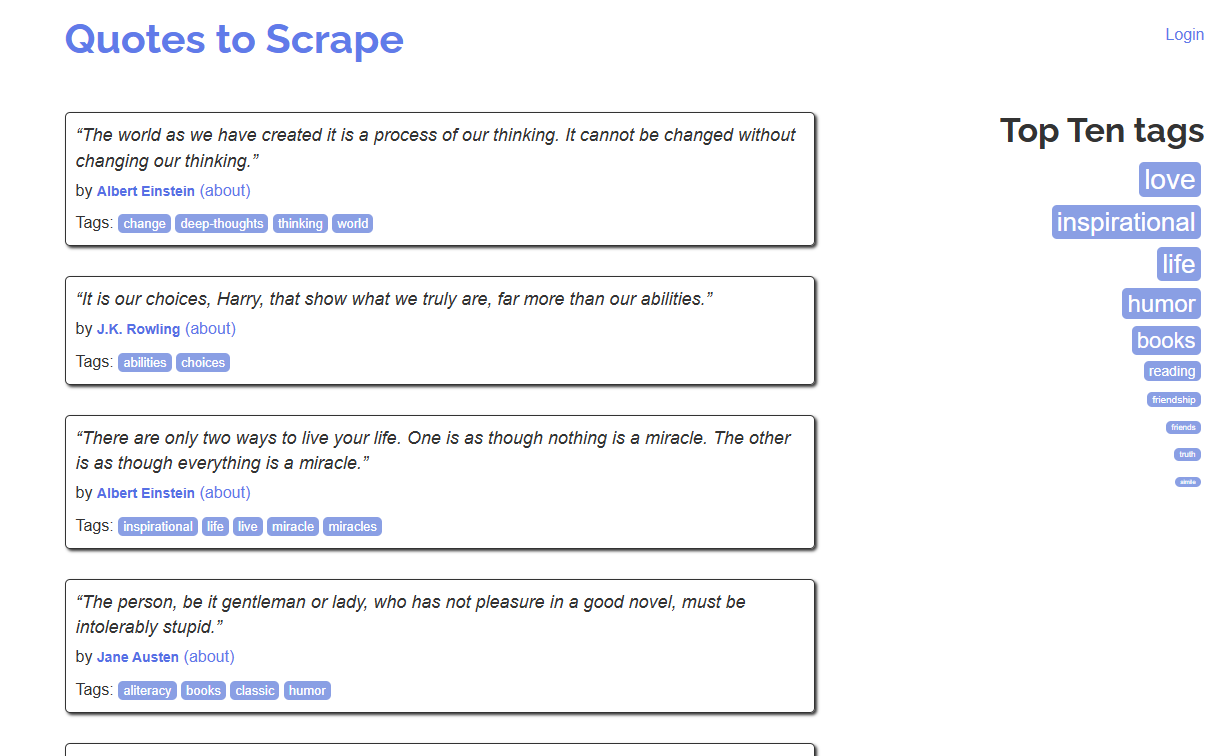
\includegraphics[width=1\columnwidth]{images/quotes-to-scrape.png}
\end{center}

\heading{HTML PRELIMINARIES}

A typical HTML element looks like the following:

\[\underbrace{\text{< h1 }}_{\text{opening tag}}\!\!\!\underbrace{\text{class = ``title">}}_{\text{attributes}}\;\underbrace{\text{My Title}}_{\text{content}}\; \underbrace{\text{</h1>}}_{\text{closing tag}}\]

HTML files are built using elements with various tags. Some common examples are:
\begin{itemize}
    \item head
    \item body
    \item header
    \item article
\columnbreak
    \item p - very common! Used for paragraphs
    \item h1,h2,...,h6 - varying heading levels (h1 is the largest)
    \item div - division/container
    \item nav - used for navigation links
    \item ul - unordered list
    \item li - a list item
    \item a - anchor (hyperlink), usually contains a ``href" attribute
    \item button
    \item table
    \item tr - a table row
    \item td - table data (a cell in a table, a child of a tr element)
\end{itemize}

For example, the following table 

\begin{center}
    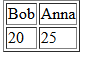
\includegraphics[width=0.25\columnwidth]{images/2x2table.png}
\end{center}

is given by the HTML:

\begin{lstlisting}[style=html]
<table border="1">
    <tr>
        <td>Bob</td>
        <td>Anna</td>
    </tr>
    <tr>
        <td>20</td>
        <td>25</td>
    </tr>
</table>
\end{lstlisting}

\columnbreak
\begin{center}
    \underline{Some ways to find HTML elements}
\end{center}

When scraping sites, we make use of the HTML elements to find the information we want. Some ways to find elements are:
\begin{enumerate}
    \item ID (this is an attribute, unique to the element)
    \item Class Name (an attribute, not unique)
    \item Tag Name (i.e. the tag of the element)
    \item XPath (see later, doesn't work with BeautifulSoup).
\end{enumerate}

\heading{IMPORTS AND INSTALLS}

Begin the script with the following imports

\begin{lstlisting}
    from bs4 import BeautifulSoup
    import requests
\end{lstlisting}

We will also need an HTML parser. For example, install \textbf{lxml} using pip.

\heading{THREE BASIC STEPS WHEN SCRAPING A SITE}

\begin{enumerate}
    \item Fetch page (makes an HTTP request to the URL and retrieves the content of the page):
    \begin{lstlisting}
        result = requests.get(my_url:str)
    \end{lstlisting}
    \item Get page content (the return above returns the HTML content and a bunch of other information, this step extracts the HTML from it)
    \begin{lstlisting}
        content = result.text
    \end{lstlisting}
    \item Create a ``Soup" (creates a BeautifulSoup object from the HTML)
    \begin{lstlisting}
        soup = BeautifulSoup(content,
                                `lxml')
    \end{lstlisting}
\end{enumerate}

\columnbreak
\heading{FINDING ELEMENTS WITH BEAUTIFULSOUP}

Once we have a ``Soup" object (called `soup' say) we can \textbf{find the first occurrence} of an HTML element by id, class or tag as follows:

\begin{itemize}
    \item by ID - finding an element by its ID attribute
    \begin{lstlisting}
        soup.find(id="example_id")
    \end{lstlisting}
    \item by Class (notice the underscore in the argument)
    \begin{lstlisting}
        soup.find(class_="example_class")
    \end{lstlisting}
    \item by Tag - pass the tag to the first argument. Unlike the other two, this is a positional argument, not a keyword argument
    \begin{lstlisting}
        soup.find("example_tag")
    \end{lstlisting}
\end{itemize}

To instead \textbf{find all occurrences} of elements with a particular property, use the find\_all method instead of find. For example:
\begin{lstlisting}
    soup.find_all(class_="example_class")
\end{lstlisting}

The find method returns BeautifulSoup objects (and find\_all returns a list of BeautifulSoup objects), so we may use the find and find\_all methods with them.\\
For example, to find the first occurrence of a table, and then find all rows in that table we can do 
\begin{lstlisting}
    table = soup.find(`table')
    rows = table.find_all(`tr')
\end{lstlisting}

To extract the text/content from a HTML element we use the get\_text method. For example, to extract the text from the main (h1) heading we do

\begin{lstlisting}
    header_text = soup.find(`h1').get_text()
\end{lstlisting}

\heading{SCRAPING MULTIPLE LINKS WITHIN A PAGE}

Often, we want to scrape a page for all links, then extract some common information from those links. This can be achieved as follows:
\begin{enumerate}
    \item Make a soup from the HTTP request.
    \item Find all anchors in the HTML using the find\_all method
    \begin{lstlisting}
        soup.find_all(`a',href=True)
    \end{lstlisting}
    \item Loop over all soup elements in the return, extracting the href from them. This is done as follows    
    \begin{lstlisting}
    for ele in soup.find_all(`a',href=True):
        ele[`href'] #some logic
    \end{lstlisting}
    \item Add some logic, usually starting with making a request and a creating a soup using the new href.
\end{enumerate}

Two warnings/things to note:
\begin{itemize}
    \item The links may be relative links, so may have to concatenate with the original URL (i.e. the root of the site).
    \item Some websites may not allow multiple requests in a short period of time. If so, ensure to \textbf{import time} and use \textbf{time.sleep(s\,:\,int)} within loops to wait `s' seconds between passes.
\end{itemize}

\heading{PAGINATION}

We can scrape sites where the information is spread over multiple pages (navigated between using a button system with a next page button). \\

With BeautifulSoup, this is somewhat ad-hoc.\\

\begin{itemize}
    \item If the "next page" HTML button element has a consistent format.
    \begin{itemize}
        \item Right-click on webpage and inspect, view the HTML of the next page button. 
        \item Commonly, this can be an anchor (tag a) inside a list item (li) inside a ul (unordered list).
    \end{itemize}
    \item Sometimes the site follows a pattern with its pages. For example "{url}?page=1", "{url}?page=2" etc. If so, this can be made use of.
\end{itemize}


\newpage
\end{multicols}

% Selenium
\begin{center}
{\huge\textbf{Selenium}}
\vspace*{0.75cm}
\end{center}

\begin{multicols}{3}
\setlength{\columnseprule}{1pt} % Add vertical line between columns

\heading{XPATH BASICS}

We will make use of XPath to scrape data from sites using Selenium, some basic syntax is as follows:

\begin{itemize}
    \item Select all elements with a certain tag via //tag\_name. \\    
    For example, //h1, //table.
    \item Select the n$^{\text{th}}$ element with a certain tag using //"tag\_name"[n] (indexing starts from 1).
    \item Select elements with a certain tag and attribute using //"tag\_name"[@Attribute\_name="value"]. E.g.
    \begin{lstlisting}[style=html]   
    //h1[@class=`main_header'].
    \end{lstlisting}
    \item There are functions such as contains() or starts-with() that can be used alongside attributes. \\
    For example, to find all h2's with class attribute value starting with `secondary' we use the following:
    \begin{lstlisting}[style=html]   
    //h2[starts-with(@class, `secondary')]
    \end{lstlisting}
    \item Special Characters:
    \begin{itemize}
        \item / - select direct children of the current element(s). \\
        For example, to select the <p> children of the <div> elements in a HTML document we can do //div/p
        \item /.. - selects the parent node of an element. \\
        For example, to obtain the parent of the first paragraph element in a document, we can do //p[1]/..
        \item * - select all direct child nodes of an element. \\
        For example, to select all siblings of a node (including itself) we can do node/../*, as this first obtains the parent of `node', and then obtains its direct children.
    \end{itemize}
\end{itemize}


\heading{IMPORTS}

Selenium is a browser automation tool, that allows us to scrape Javascript-driven sites. \\

Every script making use of selenium must have the following imports

\begin{lstlisting}[style=python]   
    from selenium import webdriver
    from selenium.webdriver.chrome.service import Service
\end{lstlisting}

\columnbreak
\heading{SETTING UP THE WEB DRIVER}

To scrape sites, a web driver must be set up. \\

As of Selenium 4.6, there is no need to download a Chrome Driver (or similar) and supply the path as an argument to the initialisation, instead, the Service import takes care of this behind the scenes.

\begin{lstlisting} 
  driver = webdriver.Chrome(service=Service())
\end{lstlisting}

To get data from a website with URL "my\_url" we do:

\begin{lstlisting}[style=python] 
    driver.get(my_url)
\end{lstlisting}

By default, this driver will open the webpage, scrape it, and close it again. This can be modified by passing some options to the initialisation of the driver. To keep the webpage open, set the options as follows:

\begin{lstlisting}[style=python]   
    options = webdriver.ChromeOptions()
    options.add_experimental_option("detach",True)
\end{lstlisting}

Alternatively, the script can be performed without displaying the webpage GUI at all. To enable this, use 
\begin{lstlisting}[style=python]            
    options.headless = True
\end{lstlisting}

Options should be passed to the ``options" kwarg of the webdriver when initilisating. e.g. 

\begin{lstlisting}[style=python] 
    driver = webdriver.Chrome(service=Service(), options=options)
\end{lstlisting}

When visiting a site using the get method of the driver, a new Chrome window will open and you will see the following message
\begin{center}
    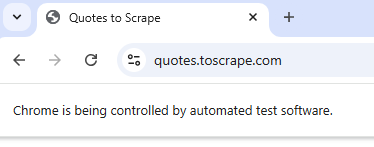
\includegraphics[width=0.9\columnwidth]{images/automated-test-software-msg.png}
\end{center}

Once you are finished scraping, ensure to close any opened windows using 
\begin{lstlisting}[style=python]   
    driver.quit()
\end{lstlisting}

\columnbreak
\heading{SCRAPING METHODS/FINDING ELEMENTS}

We can find elements using the "By" method, to use this we need to import it

\begin{lstlisting}[style=python]   
    from selenium.webdriver.common.by import By
\end{lstlisting}

We can find elements using 
\begin{itemize}
    \item ID (By.ID)
    \item Name (By.NAME)
    \item XPath (By.XPATH)
    \item Tag name (By.TAG\_NAME)
    \item Class name (By.CLASS\_NAME)
    \item CSS Selector (By.CSS\_SELECTOR)
\end{itemize}

To find elements, use the find\_element() method of the web driver. To find all occurrences of an element, use find\_elements() instead.\\

For example, to find all elements with class `author` in our test site (i.e. quotes.toscrape.com) we can do:

\begin{lstlisting}[style=python] 
    driver.find_elements(By.CLASS_NAME, "author")
\end{lstlisting}
or
\begin{lstlisting}[style=python] 
driver.find_elements(By.XPATH, "//*[@class=`author']")
\end{lstlisting}

An example of this being used is as follows:

\begin{center}
    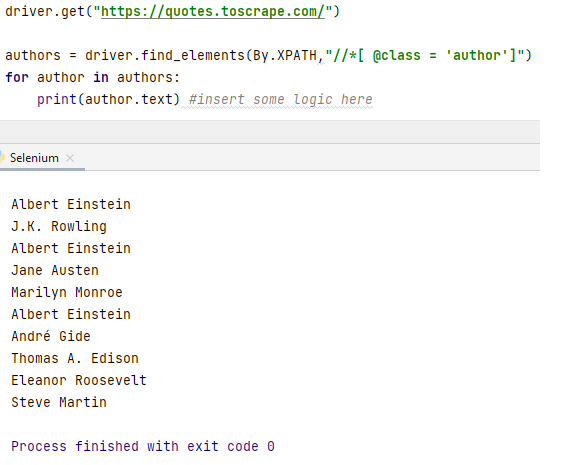
\includegraphics[width=0.9\columnwidth]{images/finding_authors_eg.png}
\end{center}

Note that the return value of driver.find\_element(...) is a WebElement object. These objects also have find\_element(s) methods and so can be used in place of "driver" to limit the scope of the search.

\heading{CLICKING A BUTTON}

To click buttons, you need a way to identify them using HTML. This could be done using tags, classes, IDs etc. \\

Once found, for example, 
\begin{lstlisting}[style=python] 
button = driver.get_element(By.ID, "next_pg_button")
\end{lstlisting}
it can be pressed using the click() method i.e. 
\begin{lstlisting}[style=python] 
    button.click()
\end{lstlisting}
In the automated browser window, you will see a new webpage load (more on how to tell the code to wait for the new webpage to load later).\\

In our test data, the next page button is a child of a list item (li) with class "next", so we press the button as follows (notice that it is the anchor tag we are clicking):

\begin{center}
    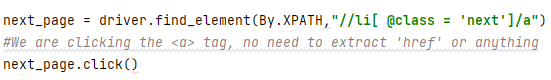
\includegraphics[width=0.9\columnwidth]{images/clicking_button.png}
\end{center}

\heading{EXTRACTING DATA FROM TABLES}

Recall that table elements are made up of tags
\begin{itemize}
    \item <tr> - a row of data.
    \item <td> - a cell of data within a row, these are children of <tr> elements.
\end{itemize}
For example, a table with one row and three columns containing data a,b,c will look as follows:
\begin{lstlisting}[style=html] 
    <table>
        <tr>
            <td>a</td>
            <td>b</td>
            <td>c</td>
        </tr>
    </table>
\end{lstlisting}

To extract all data from a table, we can do something like
\begin{lstlisting}[style=python] 
my_table = driver.find_element(By.TAG_NAME, "table")
rows = my_table.find_elements(By.TAG_NAME, "tr")
for row in rows:
    row_data = row.find_elements(By.TAG_NAME, 'td')
    #do something with the data, e.g. to print the text contents do
    print([cell.text for cell in row_data])
\end{lstlisting}

\columnbreak
\heading{SELECT AN OPTION FROM A DROPDOWN MENU}

To select from a dropdown (an element of type select or option), we need to locate it and make it a Select object. First, we need to import Select.
\begin{lstlisting}[style=python]   
    from selenium.webdriver.support.ui import Select
\end{lstlisting}

Suppose we have the following HTML 
\begin{lstlisting}[style=html]   
    <select id="dropdown">
        <option value="1">Option 1</option>
        <option value="2">Option 2</option>
        <option value="3">Option 3</option>
    </select>
\end{lstlisting}
We first locate the dropdown and make it a Select object
\begin{lstlisting}[style=python]   
    dropdown = driver.find_element(By.ID, "dropdown")
    select = Select(dropdown)
\end{lstlisting}
We can either select by visible text (using the select\_by\_visible\_text method) or by position (using the select\_by\_index method, where indexing starts from 0). \\

For example, to select Option 2 we can do either of
\begin{lstlisting}[style=python]   
    select.select_by_visible_text("Option 2")
    #or
    select.select_by_index(1)
\end{lstlisting}

\heading{IMPLICIT AND EXPLICIT WAIT TIMES}

\begin{center}
    \underline{Explicit Waits}
\end{center}

For example, "I want to wait 2 seconds after loading new pages".\\

This is achieved using the time module. For example, to wait 2 seconds in a script you would do the following:

\begin{lstlisting}[style=python]   
    import time
    time.sleep(2)
\end{lstlisting}

These waits are very easy to implement, however, they can lead to errors if the wait time is not long enough, and the next webpage has not fully loaded.

\begin{center}
    \underline{Implicit Waits}
\end{center}

These waits can be set to wait for a button to be pressable, an element to be visible etc. They are implemented using the WebDriverWait and expected\_conditions classes, as well as "By". These are imported as follows
\begin{lstlisting}[style=python]   
    from selenium.webdriver.support.ui import WebDriverWait
    from selenium.webdriver.support import expected_conditions as EC
\end{lstlisting}

\columnbreak
expected\_conditions has many available functions, some are:
\begin{itemize}
    \item element\_to\_be\_clickable \\
    The argument is a so-called locator (i.e. a way to find the element), it is a tuple, usually with a "By component" and a value. \\
    For example (By.TAG\_NAME, "my\_tag").
    \item presence\_of\_element\_located \\
    The argument is a locator (same idea as above).
\end{itemize}

An example of an implicit wait is as follows:

\begin{lstlisting}[style=python]   
WebDriverWait(driver,max_secs:int).until(EC.presence_of_element_located((By.CLASS_NAME, "my_class")))
\end{lstlisting}

This will wait for a maximum of max\_secs. It is waiting for an element with class name = "my\_class" to be located on the page.

\heading{(INFINITE) SCROLLING}

To scroll through the webpage and load the contents we make use of scrolling and returning the page height. We create a loop and keep scrolling whilst the page height keeps getting longer (as this implies new content is loading). This can be done as follows:

\begin{lstlisting}[style=python]     

    # Get initial page height
    last_height = driver.execute_script("return document.body.scrollHeight")
    
    while True:
        # Scroll down         driver.execute_script("window.scrollTo(0, document.body.scrollHeight);")
    
        # Wait for new content to load
        time.sleep(3)
    
        # Calculate new scroll height
        new_height = driver.execute_script("return document.body.scrollHeight")
    
        # Check if page height has changed
        if new_height == last_height:
            break  # If no new content, exit the loop
    
        last_height = new_height
\end{lstlisting}

\heading{ENTERING DATA}

To input data we use the send\_keys method. This is done as follows (assuming inbox\_box is the input element).

\begin{lstlisting}[style=python]     

input_box = driver.find_element(By.ID, "input_box") 

input_box.send_keys("your_username") 
\end{lstlisting}

\newpage
\end{multicols}

% Scrapy
\begin{center}
{\huge\textbf{Scrapy}}
\vspace*{0.75cm}
\end{center}

\begin{multicols}{3}
\setlength{\columnseprule}{1pt} % Add vertical line between columns

\heading{TERMINAL INPUTS AND SETUP}

Type "scrapy" in the terminal to see all available commands (start with "pip install scrapy" if needed):

\begin{center}
    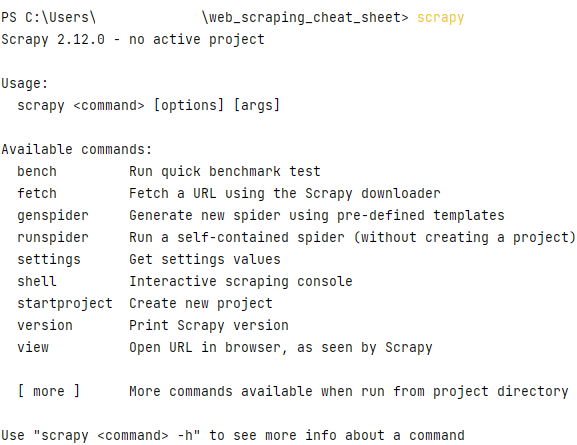
\includegraphics[width=0.9\columnwidth]{images/scrapy_commands.png}
\end{center}

To start a new project, type 

\begin{lstlisting}[style=python]     
    scrapy startproject test_project
\end{lstlisting}

(where test\_project is replaced with your project name) into the terminal, this creates a file structure as follows:

\begin{center}
    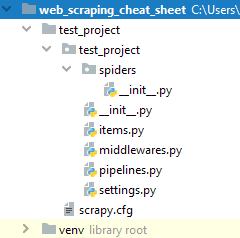
\includegraphics[width=0.4\columnwidth]{images/scrapy_project_hierarchy.png}
\end{center}

In the terminal, cd to the newly created project directory and create a new spider, you will give the spider a name and a website URL. This is done as follows:

\begin{lstlisting}[style=python]     
    cd test_project
    ...
    scrapy genspider quotes_spider https://quotes.toscrape.com/
\end{lstlisting}

\columnbreak
This creates the quotes\_spider.py file in the test\_project/spiders directory:
\begin{center}
    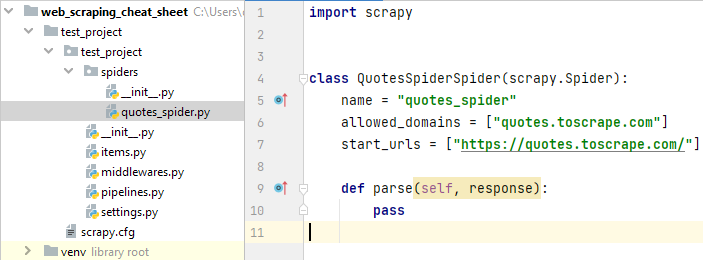
\includegraphics[width=\columnwidth]{images/created_spider.png}
\end{center}

\heading{MODIFYING AND RUNNING THE SPIDER}

To customise the spider (so it scrapes the site), we modify the parse function. \\

Note: When returning multiple pieces of data e.g. a row of a table one at a time, use `yield` instead of `return`. \\

Note: Scrapy expects the returned/yielded objects to be requests, dictionaries or None. you cannot yield a string, for example.\\

The `response` argument is a scrapy.http.Response object. We will use the .xpath() method to find elements. \\

For example, to extract the number of times each author appears on page 1 of the quotes site, we would modify the parse function to:

\begin{lstlisting}[style=python]     
def parse(self, response):
    author_count = defaultdict(int)
    for quote in response.xpath('//div[@class="quote"]'):
        author_name = quote.xpath('span/small[@class="author"]/text()').get()
        author_count[author_name] += 1
    yield author_count
\end{lstlisting}

To run the spider, go to the terminal, and whilst inside the test\_project directory, type

\begin{lstlisting}[style=python]     
    scrapy crawl quotes_spider
\end{lstlisting}

The output will be displayed to the terminal. It contains a bunch of information/logs, and amongst it you will see 

\begin{center}
    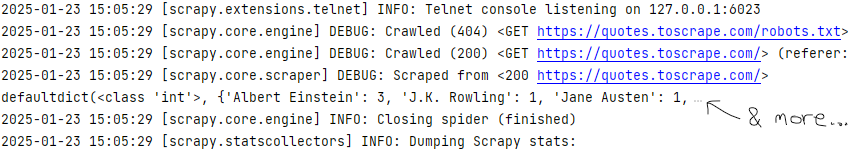
\includegraphics[width=\columnwidth]{images/scrapy_output_eg.png}
\end{center}

\heading{ABSOLUTE V.S. RELATIVE REFERENCING}

To work with relative links (e.g. "page/2/", with the whole URL being "https://quotes.toscrape.com/page/2/") there are three methods, with the latter two being preferred.

\begin{itemize}
    \item Use f-strings. \\
    If the root is stored in a variable, we can form the whole URL via 
    \begin{lstlisting}[style=python]     
    f"{root}/{relative}".
    \end{lstlisting}
    This is very prone to errors e.g. missing a slash, or having two slashes side by side.
    \item Use urljoin. For example:     
    \begin{lstlisting}[style=python]     
    response.urljoin(relative).
    \end{lstlisting}
    This handles stitching together the root and relative URLs much better.
    \item Work directly with the relative one via follow. For example: 
    \begin{lstlisting}[style=python] 
    response.follow(url=relative)
    \end{lstlisting}
\end{itemize}

\heading{SCRAPING DATA FROM LINKS (\,.FOLLOW()\,)}

We may follow and scrape the contents of links on a page using follow, moreover, we can use custom parse functions for these pages.\\

Suppose we have a relative link called `link`. We can scrape it using 
\begin{lstlisting}[style=python]     
    response.follow(url=`link',callback=self.custom_parse)
\end{lstlisting}
where custom\_parse is a custom parse function:
\begin{lstlisting}[style=python]     
    def custom_parse(self,response):
        #scrape instructions.
\end{lstlisting}

\columnbreak
\heading{SAVING TO JSON/CSV}

Currently, displaying the output of our scrapes to the terminal is not super helpful. For example, we cannot do any further data manipulation on it. \\

To do this, we simply append a command to the scrapy crawl command in the terminal. To Save to JSON or csv respectively, we do:
\begin{lstlisting}[style=python]     
    #to save to JSON
    scrapy crawl quotes_spider -o my_json.json
    #or to save to CSV
    scrapy crawl quotes_spider -o my_csv.csv
\end{lstlisting}

If we wish to add a custom column for each scraped page (something like a tag/comment), we can pass data within the `meta` argument of the `follow` method, and then retrieve it in the custom parse function.\\

The following is an example of scraping each link from the homepage of the quotes to scrape page, and tagging each scrape with the order in which they were scraped. 

\begin{center}
    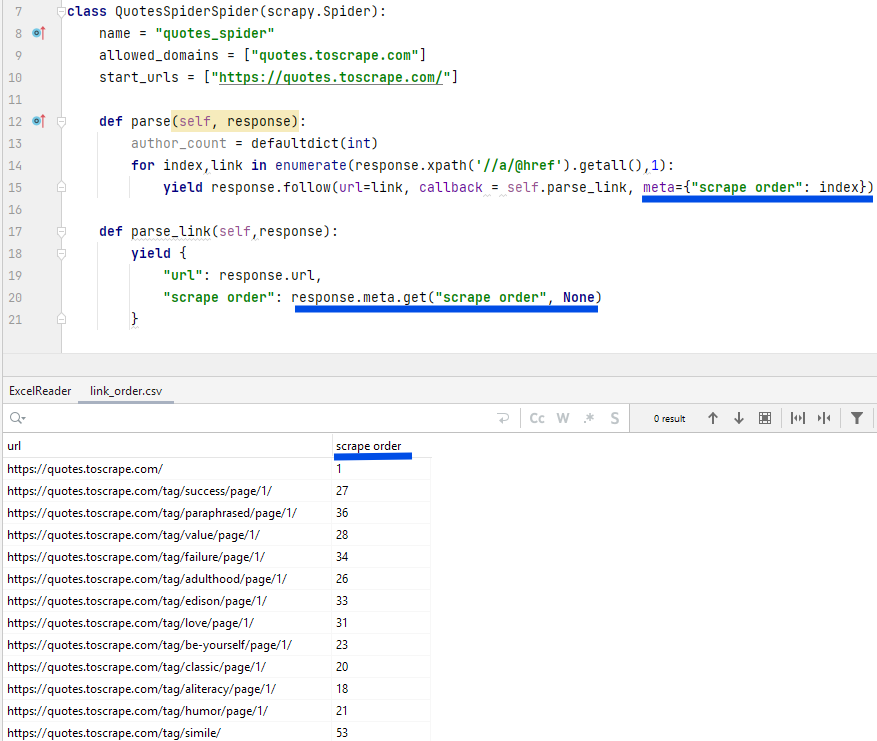
\includegraphics[width=\columnwidth]{images/meta_example.png}
\end{center}

\heading{USER AGENT}

Currently, websites we scrape know that we are using Scrapy - this is bad practice in general. We want to change this so that it looks like we are sending requests from Chrome (i.e. browsing normally).

To see the current user agent, type the following into the terminal:

\begin{lstlisting}[style=python]     
    > scrapy shell https://quotes.toscrape.com
    #wait...
    >>> request.headers
\end{lstlisting}
and within the output dictionary, there is a key called `User-Agent' containing the current user agent (by default, it will be something like `Scrapy/2.12.0 (+https://scrapy.org)').\\

We need to find a new user agent, to do this open a Chrome window and follow these steps:

\begin{itemize}
    \item Right-click and Inspect 
    \item Go to the Network tab
    \item Refresh the page
    \item Click any item in the `Name' column
    \item Find Request Headers -> User Agent
    \item e.g. Mozilla/5.0 (Linux; Android 6.0 ...
\end{itemize}

To change the user agent used by the spider:

\begin{itemize}
    \item Go to settings.py
    \item Uncomment "DEFAULT\_REQUEST\_HEADERS" (located at approximately line 40). 
    \item Add key "User-Agent", and paste the user agent copied from Chrome as the value.
\end{itemize}

\heading{EXPORT TO DATABASE}

To scrape the export the data to a database (say a SQLite3 db), we need to create a connection to SQLite3, create a table, insert scraped data into the table, and then close the connection. \\

This is done inside the `pipelines.py` file. To do this, we will create a class `SQLitePipeline` in the `pipelines.py` file, and it will have three methods, as follows:
\begin{itemize}
    \item open\_spider - This is called when the spider starts. We will use this function to setup the SQLite connection and create the table
    \item process\_item - This method will be used to insert the scraped data into the table. This method in the pipeline is called every time an item is yielded from the main parse function (or any other callback function) in your Scrapy spider. As not every yield will contain data to be inserted in the table, we should wrap the logic in try/except blocks.
    \item close\_spider - This is called when the spider ends. We will use this to close the connection to SQLite.
\end{itemize}

An example class in the pipelines.py file looks something like

\begin{lstlisting}[style=python]     
import sqlite3
import logging

class SQLitePipeline:
    def open_spider(self, spider):
        # Establish a connection to a SQLite db
        self.connection = sqlite3.connect('scrapy_data.db')
        self.cursor = self.connection.cursor()

        # Create the table if it doesn't exist
        # Use SQL syntax here 
        self.cursor.execute('''
            CREATE TABLE IF NOT EXISTS scraped_data (
                id INTEGER PRIMARY KEY AUTOINCREMENT,
                column_one TEXT,
                column_two TEXT,
                column_three TEXT
            )
        ''')
        self.connection.commit()

    def process_item(self, item, spider):
        try:
            self.cursor.execute('''
                INSERT INTO scraped_data (column_one, column_two, column_three)
                VALUES (?, ?, ?)
            ''', (item.get('field1'), item.get('field2'), item.get('field3')))
            self.connection.commit()

        # VERY IMPORTANT
        # In place of "field1", "field2", "field3", you should put the keys from the yielded dictionary in the parse function of the spider. 
        # THESE MUST MATCH EXACTLY TO AVOID ERRORS.

        except sqlite3.DatabaseError as db_error:
            #handle the error, e.g.
            logging.error(f"Database error: {db_error}")

        except Exception as e:
            # Catch any other exceptions, e.g.
            logging.error(f"Unexpected error: {e}")

        return item

    def close_spider(self, spider):
        # Close the database connection when the spider finishes
        self.connection.close()
\end{lstlisting}

Finally, inside the `settings.py` file, change the ITEM\_PIPELINES key to `SQLitePipeline` (or whatever the class is called). e.g.
\begin{lstlisting}[style=python]
    ITEM_PIPELINES = {
       "test_project.pipelines.SQLitePipeline": 300,
    }    
\end{lstlisting}
The numerical value is the priority. If multiple pipelines are being run, a lower number equals higher priority (so it will run first). This can be used to, for example, clean data (using a high-priority pipeline) before writing to a database.

\heading{SCRAPING APIS/HANDLING JSON DATA}

To see API calls from a webpage, navigate to Inspect -> Network -> Fetch/XMR. Clicking on an item in the left-hand column (may need to refresh the webpage) shows details about it.\\

To handle JSON data (i.e. if the webpage consists of JSON data, such as the return of an API request), include logic similar to the following in the parse function:

\begin{lstlisting}[style=python]
    import json 
    
    def parse(self, response):
        json_response = json.loads(response.text)
        #use `get' method to extract values. e.g.
        my_value = json_response.get("my_key")
        #...
\end{lstlisting}

\heading{LOGIN TO A WEBSITE}

To login to a website, we need to send a POST request containing the username and password to the login page.\\

For an example, we create a new spider whose start page is the login page quotestoscrape, i.e. https://quotes.toscrape.com/login , but
of course, an existing spider can also handle this, where the login data is passed to the login page via response.follow.\\

Then the idea is to extract the CSRF token using XPath or otherwise (this looks something like dGlPJRuyAbhxFjiIH...). Then send a request using FormRequest.from\_response. \\

This request should contain a callback to handle what should be done once login has occurred. The callback should start by verifying if the login was successful, for example, by checking for the existence of a logout button.\\ 

An example spider is as follows:

\begin{lstlisting}[style=python]
import scrapy
from scrapy.http import FormRequest

class QuotesLoginSpider(scrapy.Spider):
    name = 'quotes_login_spider'
    start_urls = ['https://quotes.toscrape.com/login']

    def parse(self, response):
        # Extract the CSRF token using XPath or otherwise
        csrf_token = response.xpath('//input[@name="csrf_token"]/@value').get()

        # Prepare the login data. 
        login_data = {
            "csrf_token": csrf_token,
            "username": "my_username",
            "password": "my_password",
        }
        
        yield FormRequest.from_response(
            response,  # (containing the form element)
            formdata=login_data,
            callback=self.after_login
        )    
        
    def after_login(self, response):
        # Verify login success by checking for the logout button
        if "Logout" in response.text:
            self.log("Login successful!")
            # Continue scraping here
        else:
            self.log("Login failed.")
\end{lstlisting}

Two things to note:
\begin{itemize}
    \item Scrapy will use the first form it finds in the HTML response by default. If there are multiple forms consider adding a "formxpath" key to FormRequest.from\_response to precisely locate the form.
    \item The keys in login\_data should match the `name` attributes of the `input` elements in the HTML form.
\end{itemize}

\newpage
\end{multicols}

% Splash
\begin{center}
{\huge\textbf{Splash}}
\vspace*{0.75cm}
\end{center}

\begin{multicols}{3}
\setlength{\columnseprule}{1pt} % Add vertical line between columns

Scrapy does not allow us to scrape JavaScript driven sites. For this, we need the help of Splash.

\heading{SETTING UP SPLASH WITH DOCKER}

Download and Install Docker Desktop from docker.com. You will also need WSL.\\

Install splash using the terminal (e.g. just use the one inbuilt with Docker)
\begin{lstlisting}[style=python]
    > docker pull scrapinghub/splash  
\end{lstlisting}

To run Splash in the browser, input the following command into the terminal.
\begin{lstlisting}[style=python]
    > docker run -p 8050:8050 scrapinghub/splash 
\end{lstlisting}

This can be opened in the browser with the URL
\begin{lstlisting}[style=python]
    http://localhost:8050/
\end{lstlisting}
and in the future splash can be found in the docker dashboard.\\

When opened in the browser, you see the following:

\begin{center}
    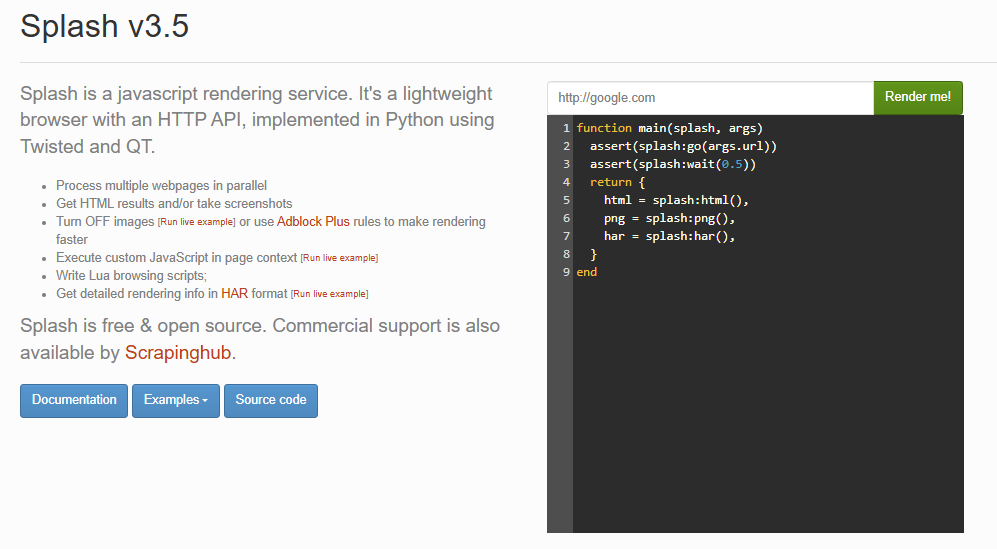
\includegraphics[width=\columnwidth]{images/splash.png}
\end{center}

\heading{USING SPLASH IN THE BROWSER}

Splash uses the Lua programming language.\\

To use, add the URL to the box above the script editor. \\

Here is an example of returning a screenshot of the quotestoscrape homepage as well as the HTML of the page. \\

Input:

\begin{center}
    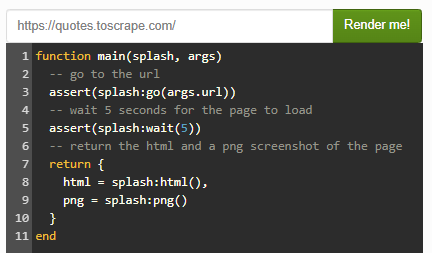
\includegraphics[width=0.8\columnwidth]{images/splash_example_input.png}
\end{center}

Output:

\begin{center}
    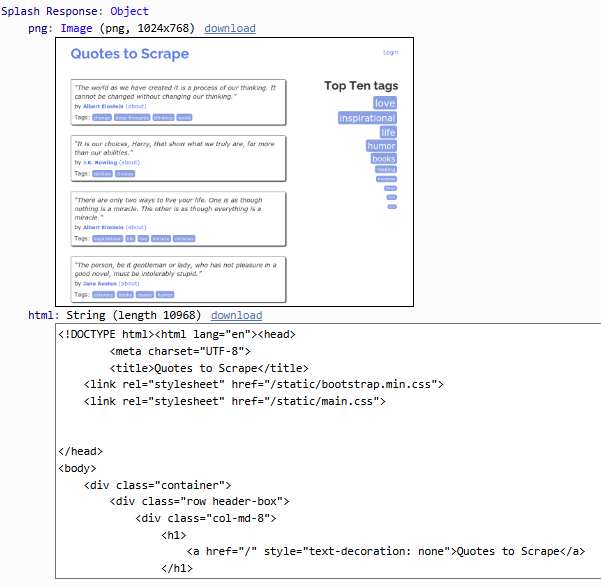
\includegraphics[width=0.9\columnwidth]{images/splash_example_output.png}
\end{center}

\heading{FINDING ELEMENTS WITH SPLASH}

HTML elements are found using CSS selector. The basics are:
\begin{itemize}
    \item Use the element name directly to find them. e.g. "p" or "div"
    \item To find elements by their ID, use \#id. For example, to find an element with id="main\_title" use `\#main\_title'.
    
    \item Similarly, use .class to find elements by their class.
\end{itemize}

To find and store an element as a variable in Splash, we do

\begin{lstlisting}[style=python]
    my_selection = assert(splash:select(<CSS selector>))
    #For example
    main_box = assert(splash:select("#main_box"))
\end{lstlisting}

Interaction with certain aspects of elements is only possible when focused on that element. To focus on an element do the following:
\begin{lstlisting}[style=python]
    my_selection:focus()
\end{lstlisting}

To input text into in input box element, do the following:

\begin{lstlisting}[style=python]
    my_input_box:send_text("my_text")
\end{lstlisting}

To click a button, do the following
\begin{lstlisting}[style=python]
    my_button:mouse_click()
\end{lstlisting}

\heading{USING SCRAPY AND SPLASH TOGETHER}

To use splash with scrapy we first need to install scrapy-splash
\begin{lstlisting}[style=python]
    > pip install scrapy-splash
\end{lstlisting}

Then we need to modify the settings.py file. This is usually a standard copy-and-paste modification, as follows:
\begin{lstlisting}[style=python]
    #In settings.py
    
    # Splash settings
    SPLASH_URL = 'http://localhost:8050'
    
    # Enable Splash's middleware
    DOWNLOADER_MIDDLEWARES = {
        'scrapy_splash.SplashCookiesMiddleware': 723,
        'scrapy_splash.SplashMiddleware': 725,
        'scrapy.downloadermiddlewares.httpcompression.HttpCompressionMiddleware': 810,
    }
    
    # Use Splash's duplicate filter
    DUPEFILTER_CLASS = 'scrapy_splash.SplashAwareDupeFilter'
    
    # Use Splash's cache storage
    HTTPCACHE_STORAGE = 'scrapy_splash.SplashAwareFSCacheStorage'
\end{lstlisting}

In the spider file (e.g. quotes\_spider.py), add a script variable within the class containing a Splash/Lua script.\\

For example, our script from before: 
\begin{lstlisting}[style=python]
  #In quotes_spider.py 
  
  script = """
    function main(splash, args)
      -- go to the url
      assert(splash:go(args.url))
      -- wait 5 seconds for the page to load
      assert(splash:wait(5))
      -- return the html and a png screenshot of the page
      return {
        html = splash:html(),
        png = splash:png()
      }
    end
  """
\end{lstlisting}

We also need to import SplashRequest, and create a `start\_requests` function which will be called before our parse function (so Splash can do any rendering of JavaScript objects before our scrapy parse function scrapes the required data).

\begin{lstlisting}[style=python]
  from scrapy-splash import SplashRequest

  def start_requests(self):
    for url in self.start_urls:
        yield SplashRequest(
            url=url,
            callback=self.parse,
            endpoint="execute",
            args={'lua_source': self.script},
        )

  #parse function defined as usual
\end{lstlisting}

\heading{CHANGE AGENT IN SPLASH}

To change the user agent, add the line 
\begin{lstlisting}[style=python]
    splash:set_user_agent("my_user_agent")
\end{lstlisting}
to the Lua script i.e. our script becomes
\begin{lstlisting}[style=python]  
  script = """
    function main(splash, args)
      splash:set_user_agent("Mozilla/5.0 (Windows NT 10.0; Win64; x64) AppleWebKit/537.36 (KHTML, like Gecko) Chrome/91.0.4472.124 Safari/537.36")
      -- go to the url
      assert(splash:go(args.url))
      -- etc...
  """
\end{lstlisting}

\newpage
\end{multicols}
\end{document}